\documentclass[12pt,a4paper]{article}
\usepackage{polski}
\usepackage{wmstitle_lic}
\usepackage{graphicx}
\usepackage{color}
\usepackage{mathtools}
\usepackage{float}
\usepackage{mathrsfs}
\usepackage{amsfonts}
\usepackage{enumerate}
\usepackage{amsthm}

\newtheorem{df}{Definicja}[section]
\newtheorem{pr}{Przyk{\l}ad}[section]
\newtheorem{twr}{Twierdzenie}[section]
\newtheorem{pro}{Problem}[section]
\newtheorem{wn}{Wniosek}[section]

\begin{document}

\title{Hipoteza \v Cernego}
\author{Sylwia Klimkiewicz, Adam Jamka}
\promotor{Wit Fory\'s}
\nralbumu{276782, 276765}
\maketitle

\section*{Wst\k{e}p}
W poni\.{z}szej pracy przedstawimy Hipotez\k{e} \v Cernego oraz zwi\k{a}zane z ni\k{a} zagadnienia. Problem ten dotyczy teorii automat\'ow i jest zwi\k{a}zany z ograniczeniem d{\l}ugo\'{s}ci s{\l}owa synchronizuj\k{a}cego dany automat. Jest to problem otwarty ju\.{z} od ponad 45 lat. Praca zosta{\l}a napisana na potrzeby uko\'{n}czenia studi\'{o}w. Pierwszy rozdzia{\l} jest dzie{\l}em pracy wsp\'{o}lnej, rozdzia{\l}y 2, 3 oraz 4 s\k{a} autorstwa Adama Jamki, natomiast rozdzia{\l}y 5, 6, 7 Sylwii Klimkiewicz.

%% SEKCJA 1 Podstawowe definicje
\section{Podstawowe definicje i twierdzenia.}
%% def 1.1
\begin{df} 
Grafem nazywamy par\k{e} $G=(V,E)$, gdzie $V$ jest niepustym zbiorem, kt\'orego elementy zwane s\k{a} wierzcho{\l}kami, a $E$ jest rodzin\k{a} dwuelementowych podzbior\'ow zbioru $V$, zwanych kraw\k{e}dziami.
$E=\{vw : v,w\in V \}$.
\end{df}
%% def 1.2
\begin{df} 
Niech $G=(V,E)$ b\k{e}dzie grafem. Liczb\k{e} wierzcho{\l}\'ow grafu $G$ nazywamy rz\k{e}dem grafu i oznaczamy $|V|$, natomiast liczb\k{e} kraw\k{e}dzi nazywamy rozmiarem grafu i oznaczamy $|E|$.
\end{df}
%% def 1.3
\begin{df} 
Niech $G=(V,E)$ b\k{e}dzie grafem. Zbi\'or s\k{a}siad\'ow wierzcho{\l}ka $v\in V$ $N(v)$ sk{\l}ada si\k{e} z wszystkich wierzcho{\l}k\'ow grafu $G$, takich \.ze istniej\k{a} kraw\k{e}dzie nale\.z\k{a}ce do zbioru $E$, {\l}\k{a}cz\k{a}ce te wierzcho{\l}ki z v. $N(v)=\{w : vw\in E\}$.
\end{df} 
%% def 1.4
\begin{df} 
Niech $G=(V,E)$ b\k{e}dzie grafem. Stopniem wierzcho{\l}ka $v\in V$ nazywamy liczb\k{e} jego s\k{a}siad\'ow i oznaczamy $deg(v)$.
\end{df}
%% def 1.5
\begin{df} 
Graf $G=(V,E)$ jest r-regularny, je\.zeli wszystkie jego wierzcho{\l}ki maj\k{a} stopie\'n r\'owny r.
\end{df} 
%% def 1.6
\begin{df} 
Iloczynem kartezja\'nskim zbior\'ow $A$ i $B$ nazywamy zbi\'or wszystkich par uporz\k{a}dkowanych $(a,b)$ gdzie $a\in A, b\in B$ i oznaczamy $A\times B$ 
\end{df}
%% def 1.7 
\begin{df} 
Kraw\k{e}dzi\k{a} skierowan\k{a} grafu $G=(V,E)$ nazywamy element zbioru $V\times V$.
\end{df}
%% def 1.8
\begin{df} 
Graf sk{\l}adaj\k{a}cy si\k{e} tylko z kraw\k{e}dzi skierowanych nazywamy grafem skierowanym.
\end{df}
%% def 1.9
\begin{df} 
Niech $G=(V,E)$ b\k{e}dzie grafem. Ci\k{a}g wierzcho{\l}k\'ow $(v_{1}, \ldots, v_{n})$, taki \.ze $\forall_{i}$ $v_{i}\in V$ oraz  $v_{i-1}v_{i} \in E$ dla $i=2, \ldots, n$ nazywamy \'scie\.zk\k{a} w grafie $G$.
\end{df} 
%% def 1.10
\begin{df} 
Graf $G$ jest sp\'ojny je\'sli dowolne dwa jego wierzcho{\l}ki s\k{a} po{\l}\k{a}czone \'scie\.zk\k{a}.
\end{df}
%% def 1.11
\begin{df} 
Automatem nazywamy tr\'{o}jk\k{e} $\mathscr{A}=(Q, \Sigma, \delta)$, gdzie Q jest zbiorem mo\.{z}liwych stan\'{o}w, $\Sigma$ jest alfabetem, natomiast $\delta:Q \times \Sigma \rightarrow$ Q jest funkcj\k{a} okre\'{s}laj\k{a}c\k{a} zachowanie si\k{e} automatu pod wp{\l}ywem litery nale\.{z}\k{a}cej do alfabetu $\Sigma$ w stanie q \in Q.
\end{df}
%% wn 1.1 
\begin{wn}
Automat $\mathscr{A}=(Q, \Sigma, \delta)$ mo\.zemy interpretowa\'c jako graf skierowany, w kt\'orym $Q$ jest zbiorem wierzcho{\l}k\'ow, a odwzorowanie $\delta$ okre\'sla kraw\k{e}dzie gafu, kt\'ore dodatkowo s\k{a} poetykietowane literami alfabetu $\Sigma$.
\end{wn}
%% def 1.12
\begin{df} 
S{\l}owem resetuj\k{a}cym lub synchronizuj\k{a}cym automat nazywamy s{\l}owo $\omega \in \Sigma$ takie, \.{z}e dla dowolonych stan\'{o}w $q, q' \in Q$ automatu $\mathscr{A}=(Q, \Sigma, \delta)$ zachodzi $\delta(q,w)=\delta(q',w)$
\end{df}
%% def 1.13
\begin{df} 
Automat $\mathscr{A}=(Q, \Sigma, \delta)$ nazywamy synchronicznym je\'{s}li istnieje s{\l}owo $\omega \in \Sigma$ synchronizuj\k{a}ce ten automat.
\end{df}
%% def 1.14 
\begin{df}
Problem NP to problem decyzyjny, w kt\'orym sprawdzenie poprawno\'sci rozwi\k{a}zania wymaga z{\l}o\.zono\'sci obliczeniowej wielomianowej, a znalezienie rozwi\k{a}zania wymaga z{\l}o\.zono\'sci co najmniej wielomianowej.
\end{df}
%% def 1.15
\begin{df}
Problem NP-trudny to problem obliczeniowy, dla kt\'orego nie mo\.zna znale\'z\'c rozwi\k{a}zania w czasie wielomianowym, a sprawdzenie poprawno\'sci rozwi\k{a}zania jest co najmniej tak trudne jak ka\.zdego innego problemu z klasy NP.
\end{df}
%% def 1.16 
\begin{df}
Problm NP-zupe{\l}ny to problem decyzyjny dla kt\'orego nie mo\.zna znale\'z\'c rozwi\k{a}zania w czasie wielomianowym, natomiast sprawdzenie poprawno\'sci rozwi\k{a}zania jest mo\.zliwe w czasie wielomianowym. 
\end{df}
%% def 1.17
\begin {df} 
Problem coNP to problem nale\.z\k{a}cy do klasy problem\'ow dope{\l}niaj\k{a}cych problemy NP.
\end{df}
%% def 1.18
\begin{df}
Problem PSPACE to problem decyzyjny, dla kt\'orego mo\.zna znale\'z\'c rozwi\k{a}zanie wykorzystuj\k{a}c przestrze\'n wielomianow\k{a}.
\end{df}
%% def 1.19
\begin{df} 
Elementem neutralnym dzia{\l}ania $+:K\times K\rightarrow K$ nazywamy $e\in K$, takie \.ze $\forall_{x\in K}:e+x=x+e=x$.
\end{df}
%% def 1.20 
\begin{df} 
Par\k{e}$(K,+)$, gdzie $K$ jest zbiorem, a $+$ jest dzia{\l}aniem okre\'slonym w $K$ nazywamy grup\k{a}, je\.zeli spe{\l}nione s\k{a} nast\k{e}puj\k{a}ce warunki:
\begin{enumerate}[I.]
\item $+: K\times K \rightarrow K$
\item $\forall_{x,y,z\in K}: (x+y)+z=x+(y+z)$
\item $\exists_{e\in K} \forall_{x\in K}: x+e=e+x=x$ 
\item $\forall_{x\in K} \exists_{x'\in K}: x+x'=x'+x=e$
\end{enumerate}
\end{df}
%% def 1.21 
\begin{df} 
Grup\k{e} $(K,+)$ nazywamy abelow\k{a} lub przemienn\k{a}, je\.zeli $\forall_{x,y\in K}: x+y=y+x$.
\end{df}
%% def 1.22 
\begin{df} 
Tr\'ojk\k{e} $(K,+,*)$ gdzie K jest zbiorem, a $+$ i $*$ s\k{a} dzia{\l}aniami okre\'slonymi w $K$ nazywamy pier\'scieniem, je\.zeli spe{\l}nione s\k{a} nast\k{e}puj\k{a}ce warunki:
\begin{enumerate}[I.]
\item $(K,+)$ jest grup\k{a} abelow\k{a} 
\item $*:K\times K \rightarrow K$ 
\item $\forall_{x,y,z\in K}: (x*y)*z=x*(y*z)$
\item $\forall_{x,y,z\in K}: (x+y)*z=(x*z)+(y*z)$ oraz $x*(y+z)=(x*y)+(x*z)$
\end{enumerate}
Dzia{\l}anie $+$ nazywamy dzia{\l}aniem addytywnym, natomiast $*$ nazywamy dzia{\l}aniem multiplikatywnym.
\end{df}
%% def 1.23 
\begin{df} 
Pier\'scie\'n (K,+,*) nazywamy pier\'scieniem z jedno\'sci\k{a} je\.zeli istnieje $e'\in K$ taki, \.ze $\forall_{x\in K}: e'*x=x*e'=x$. W\'owczas $e'$ jest elementem neutralnym dzia{\l}ania $*$.
\end{df}
%% def 1.24 
\begin{df} 
Pier\'scie\'n z jedno\'sci\k{a} (K,+,*) nazywamy cia{\l}em, je\.zeli $\forall_{x\in K-\{e\}} \exists_{x^{-1}\in K}: x^{-1}*x=e'$, gdzie $e$ jest elementem neutralnym działania $+$.
\end{df}
%% def 1.25
\begin{df}
Przestrzeni\k{a} liniow\k{a} lub wektorow\k{a} nad cia{\l}em $K$ nazywamy $(V, +, *)$, gdzie $V$ jest niepustym zbiorem oraz spe{\l}nia nast\k{e}puj\k{a}ce warunki:
\begin{enumerate}[I.]
\item $\forall_{u, v, w \in V}: u + (v + w) = (u + v) + w$
\item $\forall_{v, w \in V}: v + w = w + v$
\item $\exists_{0 \in V} \forall_{v \in V}: v + 0 = v$
\item $\forall_{v \in V} \exists_{w \in V}: v + w = 0$
\item $\forall_{\alpha \in K} \forall_{v, w \in V}: \alpha(v + w) = \alpha v + \alpha w$
\item $\forall_{\alpha, \beta \in K} \forall_{v \in V}: (\alpha + \beta)v = \alpha v + \beta v$
\item $\forall_{\alpha, \beta \in K} \forall_{v \in V}: \alpha(\beta v) = (\alpha*\beta)v$
\item $\exists_{1 \in K} \forall_{v \in V}: 1v = v$
\end{enumerate}
\end{df}
%% def 1.26
\begin{df}
Niech $(V,+,*)$ b\k{e}dzie przestrzeni\k{a} wektorow\k{a} nad cia{\l}em $K$. Wektory $v_{1}, v_{2}, \dots, v_{n}\in V$ s\k{a} liniowo niezale\.{z}ne wtedy i tylko wtedy, gdy $\forall_{\alpha_{1}, \alpha_{2}, \dots, \alpha_{n} \in K} \alpha_{1}v_{1} + \alpha_{2}v_{2} + \dots + \alpha_{n}v_{n} = 0 => \alpha_{1} = \alpha_{2} = \dots = \alpha_{n} = 0$
\end{df}
%% def 1.27 
\begin{df}
Niech $(V, +, *)$ b\k{e}dzie przestrzeni\k{a} wektorow\k{a} nad cia{\l}em $K$, $A\subseteq V$. Zbi\'or $spanA=\{v\in V: v=\alpha_{1}v_{1}+\ldots+\alpha_{k}v_{k}: \alpha_{1},\ldots,\alpha_{k}\in K, v_{1},\ldots,v_{k}\in A\}$ nazywamy pow{\l}ok\k{a} liniow\k{a} zbioru $A$.
\end{df}
%% def 1.28
\begin{df}
Niech $(V, +, *)$ b\k{e}dzie przestrzeni\k{a} wektorow\k{a} nad cia{\l}em $K$. Podzbi\'or $U$ przestrzeni $V$ nazywamy podprzestrzeni\k{a} wekorow\k{a} lub liniow\k{a} wtedy i tylko wtedy, gdy spe{\l}nione s\k{a} nast\k{e}puj\k{a}ce warunki:
\begin{enumerate}[I.]
\item $\forall_{u,v\in U}: u+v\in U$ 
\item $\forall_{\alpha\in K}\forall_{u\in U}: \alpha u\in U$
\end{enumerate}
\end{df}
%% wn 1.2
\begin{wn}
Podzbi\'or $U$ przestrzeni wektorowej $V$ nad cia{\l}em $K$ jest podprzestrzeni\k{a} wektorow\k{a} wtedy i tylko wtedy, gdy $(U, +, *)$ jest przestrzeni\k{a} wektorow\k{a} nad cia{\l}em $K$.
\end{wn}
%% def 1.29 baza przestrzeni
\begin{df}
Niech $(V, +, *)$ b\k{e}dzie przestrzeni\k{a} wektorow\k{a} nad cia{\l}em $K$. Zbi\'{o}r $B \subset V$ nazywamy baz\k{a} przestrzeni $V$ je\'{s}li:
\begin{enumerate}[I.]
\item $span B = V$ (zbi\'{o}r $B$ generuje ca{\l}\k{a} przestrze\'{n} $V$, czyli ka\.{z}dy wektor $v \in V$ daje si\k{e} zapisa\'{c} jako sko\'{n}czona kombinacja liniowa wektor\'{o}w z $B$)
\item $B$ jest zbiorem wektor\'{o}w liniowo niezale\.{z}nych.
\end{enumerate}
\end{df}
%% def 1.30 wymiar przestrzeni
\begin{df}
Niech $B$ b\k{e}dzie dowolna baz\k{a} przestrzeni wektorowej $V$:
\begin{itemize}
\item Je\'{s}li $B$ jest zbiorem sko\'{n}czonym ($\#B<\infty$) to m\'{o}wimy, \.{z}e przestrze\'{n} $V$ jest sko\'{n}czenie wymiarowa, a liczb\k{e} wektor\'{o}w w bazie $B$ nazywamy wymiarem przestrzeni i oznaczmy $dim V$
\item Je\'{s}li $B$ sk{\l}ada si\k{e} z niesko\'{n}czonej liczby wektor\'{o}w to m\'{o}wimy, \.{z}e $V$ jest niesko\'{n}czenie wymiarowa i piszemy $dim V = \infty$
\item Je\'{s}li $V =$ \{\={0}\} przyjmujemy $dim V = 0$
\end{itemize}
\end{df}
%% def 1.31 standardowy iloczyn skalarny
\begin{df}
Standardowym iloczynem skalarnym $u = (u_{1}, \dots, u_{n}) \in R^{n}$ oraz $v = (v_{1}, \dots, v_{n}) \in R^{n}$ nazywamy liczb\k{e} $<u, v> := \sum_{i=1}^{n} u_{i}v_{i} = u_{1}v_{1} + \dots + u_{n}v_{n}$
\end{df}
%% df 1.32 wektor normalny
\begin{df}
Wektorem normalnym nazywamy wektor prostopad{\l}y do danej przestrzeni.
\end{df}
%% twierdzenie 1.1
\begin{twr}
(WKW na podprzestrze\'{n} wektorow\k{a}) \newline Niech  $(V, +, *)$ - przestrze\'{n} wektorowa nad cia{\l}em $K$. Zbi\'{o}r $U \subset V$ jest podprzestrzeni\k{a} wektorow\k{a} przestrzeni $V \Leftrightarrow \forall_{\alpha, \beta \in K} \forall_{u, v \in U} \alpha u + \beta v \in U$.
\end{twr}
\begin{proof}
$(=>)$ Zak{\l}adam, \.{z}e zbi\'{o}r $U \subset V$ jest podprzestrzeni\k{a} wektorow\k{a}. We\'{z}my dowolne $\alpha, \beta \in K$ oraz $u, v \in U => \alpha u \in U$ oraz $\beta v \in U => \alpha u + \beta v \in U$
\newline
$(<=)$ Zak{\l}adam, \.{z}e $\forall_{\alpha, \beta \in K} \forall_{u, v \in U} \alpha u + \beta v \in U$.
\begin{itemize}
\item Czy $\forall_{u, v \in U} => u+v \in U$? Tak, poniewa\.{z} wystarczy w za{\l}o\.{z}eniach przyj\k{a}\'{c} $\alpha = \beta = 1$, a wtedy $1*u+1*v \in U => u + v \in U$
\item Czy $\forall_{\alpha \in K} \forall_{u \in U} => \alpha u \in U$? Tak, poniewa\.{z} przy przyj\k{e}tych za{\l}o\.{z}eniach we\'{z}miemy $\beta = 0$ oraz $v =$ \={0}. W\'{o}wczas otrzymujemy $\alpha u + 0 *$\={0} $= \alpha u \in U$
\end{itemize}
\end{proof}

%% twierdzenie 1.2
\begin{twr}
$Span A$ jest podprzestrzeni\k{a} wektorow\k{a} w $V$ i do tego jest to najmniejsza podprzestrze\'{n} wektorowa $V$ zawieraj\k{a}ca zbi\'{o}r A.
\end{twr}
\begin{proof}
$Span A$ jest podprzestrzeni\k{a} wektorow\k{a}, poniewa\.{z} \newline $\forall_{u, v \in span A} \forall_{\alpha, \beta \in K} \exists_{u_{1}, \dots, u_{k} \in A}$ $ \exists_{\alpha_{1}, \dots, \alpha_{k} \in K}$ $u = \alpha_{1}u_{1} + \dots + \alpha_{k}u_{k} \exists_{v_{1}, \dots, v_{k} \in A} \exists_{\beta_{1}, \dots, \beta_{k} \in K} v = \beta_{1}v_{1}  + \dots + \beta_{k}v_{k}$, a wi\k{e}c $\alpha u + \beta v = \alpha (\alpha_{1}u_{1} + \dots + \alpha_{k}u_{k}) + \beta (\beta_{1}v_{1} + \dots + \beta_{k}v_{k}) = \alpha \alpha_{1}u_{1}  + \dots + \alpha \alpha_{k}u_{k} + \beta \beta_{1}v_{1} + \dots + \beta \beta_{k}v_{k} \in span A$ \newline
Niech $W \subset V$ - podprzestrze\'{n} wektorowa w $V$ taka, \.{z}e $A \subset W$. Wystarczy pokaza\'{c}, \.{z}e $span A \subset W$.
\end{proof}

%% SEKCJA 2 Wprowadzenie do problemu
\section{Wprowadzenie do problemu. Przyk{\l}ady zastosowa\'{n}.}

%%Przykład 2.1
\begin{pr}
\label{pr:przyklad1}
Przyk{\l}adem synchronicznego automatu  $\mathscr{A}$ z czterema stanami Q = \textbraceleft 1, 2, 3, 4\textbraceright  oraz alfabetem sk{\l}adaj\k{a}cym si\k{e} z dw\'{o}ch liter $\Sigma$ = \textbraceleft a, b\textbraceright  mo\.{z}e by\'c poni\.{z}szy graf.
%% Rysunek 1
\begin{figure}[H]
    \centering
    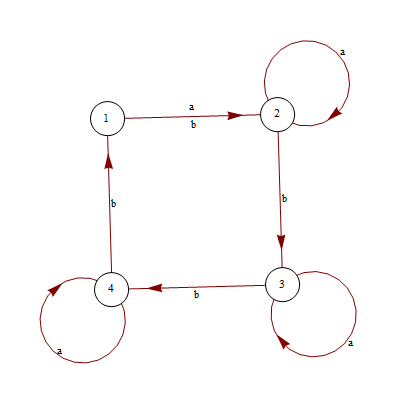
\includegraphics[width=0.62\textwidth]{rysunek1}
    \caption{Synchroniczny automat}
    \label{fig:rysunek1}
\end{figure}

{\L}atwo mo\.{z}emy sprawdzi\'{c}, \.{z}e s{\l}owem resetuj\k{a}cym automat na rysunku \ref{fig:rysunek1} jest \textit{abbbabbba}, co r\'{o}wnowa\.{z}nie mo\.{z}emy zapisa\'{c} \textit{a$b^{3}$a$b^{3}$a}. Pos{\l}ugujac si\k{e} tym s{\l}owem, niezale\.{z}nie od stanu pocz\k{a}tgowego, \'{s}cie\.{z}ka zawsze sko\'{n}czy si\k{e} na wierzcho{\l}ku drugim.\\
\\
\textbf{1}$\xrightarrow{a}$2$\xrightarrow{b}$3$\xrightarrow{b}$4$\xrightarrow{b}$1$\xrightarrow{a}$2$\xrightarrow{b}$3$\xrightarrow{b}$4$\xrightarrow{b}$1$\xrightarrow{a}$\textbf{2}\\
\textbf{2}$\xrightarrow{a}$2$\xrightarrow{b}$3$\xrightarrow{b}$4$\xrightarrow{b}$1$\xrightarrow{a}$2$\xrightarrow{b}$3$\xrightarrow{b}$4$\xrightarrow{b}$1$\xrightarrow{a}$\textbf{2}\\
\textbf{3}$\xrightarrow{a}$3$\xrightarrow{b}$4$\xrightarrow{b}$1$\xrightarrow{b}$2$\xrightarrow{a}$2$\xrightarrow{b}$3$\xrightarrow{b}$4$\xrightarrow{b}$1$\xrightarrow{a}$\textbf{2}\\
\textbf{4}$\xrightarrow{a}$4$\xrightarrow{b}$1$\xrightarrow{b}$2$\xrightarrow{b}$3$\xrightarrow{a}$3$\xrightarrow{b}$4$\xrightarrow{b}$1$\xrightarrow{b}$2$\xrightarrow{a}$\textbf{2}
\end{pr}

Rozwa\.{z}my teraz troszk\k{e} bardziej rozbudowany automat, tak zwany automat Ashby. Przyk{\l}ad ten opisuje jak poradzi\'{c} sobie ze st{\l}umieniem ha{\l}asu generowanego przez dwa \'{z}r\'{o}d{\l}a - \'{s}piew oraz \'{s}miech.

%% Przykład 2.2
\begin{pr}
W tym automacie mamy tyle samo stan\'{o}w co w Przyk{\l}adzie \ref{pr:przyklad1}  Q = \textbraceleft 00, 01, 10, 11\textbraceright, lecz ilo\'{s}\'{c} liter w alfabecie zosta{\l}a zwi\k{e}kszona do czterech $\Sigma$ = \textbraceleft a, b, c, d\textbraceright. Ka\.{z}dy stan sk{\l}ada si\k{e} z dw\'{o}ch cyfr, pierwsza b\k{e}dzie odpowiada{\l}a za ha{\l}as generowany przez \'{s}piew, a druga przez \'{s}miech, gdzie \textit{0} oznacza\'{c} b\k{e}dzie brak ha{\l}asu, natomiast \textit{1} generowanie nieprzyjemnego d\'{z}wi\k{e}ku.

%% Rysunek 2
\begin{figure}[H]
    \centering
    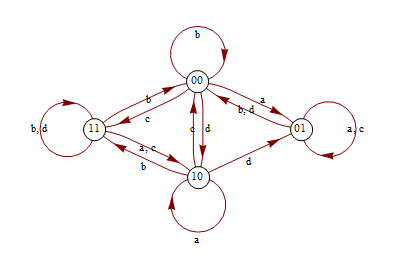
\includegraphics[width=1.05\textwidth]{rysunek2}
    \caption{Automat Ashby}
    \label{fig:rysunek2}
\end{figure}

Rozwa\.{z}aj\k{a}c s{\l}owo \textit{acb} stwierdzimy, \.{z}e jest ono s{\l}owem resetuj\k{a}cym automat przedstawiony na Rysunku \ref{fig:rysunek2}.\\
\\
\textbf{00}$\xrightarrow{a}$01$\xrightarrow{c}$01$\xrightarrow{b}$\textbf{00}\\
\textbf{01}$\xrightarrow{a}$01$\xrightarrow{c}$01$\xrightarrow{b}$\textbf{00}\\
\textbf{10}$\xrightarrow{a}$10$\xrightarrow{c}$00$\xrightarrow{b}$\textbf{00}\\
\textbf{11}$\xrightarrow{a}$01$\xrightarrow{c}$00$\xrightarrow{b}$\textbf{00}\\

Oznacza to, i\.{z} po zastosowaniu tego s{\l}owa ha{\l}as nie b\k{e}dzie generowany ani przez \'{s}piew, ani przez \'{s}miech, a wi\k{e}c b\k{e}dziemy w stanie do kt\'{o}rego d\k{a}\.{z}yli\'{s}my.
\end{pr}

Po przeanalizowaniu powy\.{z}szych przyk{\l}ad\'{o}w dochodzimy do wniosku, i\.{z} po zastosowaniu s{\l}owa resetuj\k{a}cego ko\'{n}czymy prac\k{e} w znanym z g\'{o}ry stanie, lecz nie wiemy z kt\'{o}rego stanu zaczynali\'{s}my.

Nast\k{e}pny przyk{\l}ad poka\.{z}e jakie zastosowanie mo\.{z}e dany problem mie\'{c} w dziedzinie przemys{\l}u, handlu, gdzie np. b\k{e}dziemy pakowa\'{c} jakie\'{s} elementy, kt\'{o}re maj\k{a} okre\'{s}lony kszta{\l}t.

%% Przykład 2.3
\begin{pr}
Przypu\'{s}\'{c}my, \.{z}e nasz przedmiot ma kszta{\l}t wielok\k{a}ta przedstawionego na Rysunku \ref{fig:rysunek3}.

%% Rysunek 3
\begin{figure}[H]
    \centering
    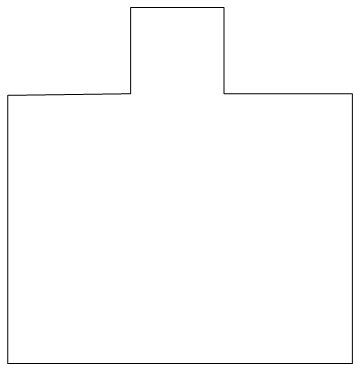
\includegraphics[width=0.23\textwidth]{rysunek3}
    \caption{Wielok\k{a}tny element}
    \label{fig:rysunek3}
\end{figure}


Ka\.{z}dy taki element wk{\l}adamy do pude{\l}ka, lecz zanim to zrobimy musimy je odpowiednio posortowa\'{c}, tak aby mia{\l}y t\k{a} sam\k{a} orientacj\k{e}. Dla u{\l}atwienia przypu\'{s}my, \.{z}e s\k{a} mo\.{z}liwe tylko cztery pozycje tego elementu, kt\'{o}re s\k{a} widoczne na Rysunku \ref{fig:rysunek4}.

%% Rysunek 4
\begin{figure}[H]
    \centering
    
\includegraphics[width=0.87\textwidth]{rysunek4}
    \caption{Mo\.{z}liwe orientacje elementu}
    \label{fig:rysunek4}
\end{figure}

Za{\l}\'{o}\.{z}my, \.{z}e interesuj\k{a}ca dla nas jest druga od lewej strony orientacja elementu. Skorzystamy z lekko zmodyfikowanego automatu, kt\'{o}ry juz wcze\'{s}niej poznali\'{s}my, a dok{\l}adniej z automatu przedstawionego na Rysunku \ref{fig:rysunek1}. G{\l}\'{o}wna zmiana b\k{e}dzie polega{\l}a na tym, i\.{z} mo\.{z}liwe stany, kt\'{o}re automat mo\.{z}e przyj\k{a}\'{c} b\k{e}d\k{a} kolejnymi orientacjami tego elementu.
\\
%% Rysunek 5
\begin{figure}[H]
    \centering
    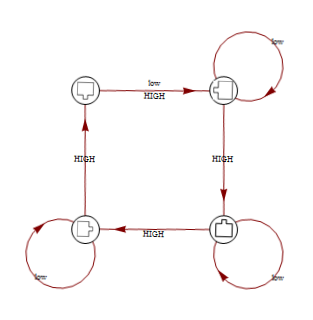
\includegraphics[width=0.7\textwidth]{rysunek5}
    \caption{Zmiana orientacji elementu}
    \label{fig:rysunek5}
\end{figure}

Pami\k{e}taj\k{a}c s{\l}owo resetuj\k{a}ce w automacie z Rysunku \ref{fig:rysunek1} abbbabbba wnioskujemy, \.{z}e s{\l}owem resetuj\k{a}cym automat na Rysunku \ref{fig:rysunek5} jest low-HIGH-HIGH-HIGH-low-HIGH-HIGH-HIGH-low, a stan ko\'{n}cowy to orientacja elementu, kt\'{o}r\k{a} chcieli\'{s}my uzyska\'{c}.
\end{pr}

Jak wida\'{c} nawet dla ma{\l}o skomplikowanego automatu synchronicznego mo\.{z}emy znale\'{z}\'{c} proste, a przede wszystkim z \.{z}ycia wzi\k{e}te zastosowanie, kt\'{o}re oczywi\'{s}cie mo\.{z}emy uog\'{o}lnia\'{c}, a sam automat stara\'{c} si\k{e} rozwija\'{c}, powi\k{e}ksza\'{c}.


%% SEKCJA 3 Algorytm znajdowania słowa sychronizującego
\section{Algorytm znajdowania s{\l}owa synchronizuj\k{a}cego.}

Za{\l}\'{o}\.{z}my, \.{z}e mamy dany automat  $\mathscr{A}=(Q, \Sigma, \delta)$. Konstruujemy automat pot\k{e}gowy $P(\mathscr{A})$. Jego zbi\'{o}r stan\'{o}w to zbi\'{o}r $P'(Q)$, kt\'{o}ry jest niepustym podzbiorem Q, a funkcja przejscia $\delta$ jest naturalnie rozszerzona do zbioru $P'(Q)\times \Sigma$. Inaczej m\'{o}wi\k{a}c dla ka\.{z}dego niepustego podzbioru $P$ zbioru $Q$ oraz $a \in \Sigma$ mamy $\delta(P,a)=\{\delta(p,a) | p \in P\}$.
\\
%% Rysunek 6
\begin{figure}[H]
    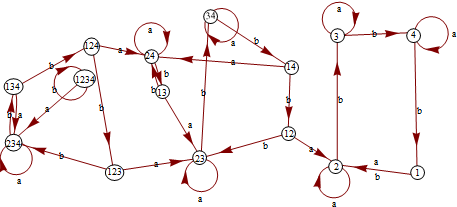
\includegraphics[width=1.1\textwidth]{rysunek6}
    \caption{Automat pot\k{e}gowy}
    \label{fig:rysunek6}
\end{figure}

Na Rysunku \ref{fig:rysunek6} przedstawiony zosta{\l} automat pot\k{e}gowy dla sko\'{n}czonego automatu przedstawionego na Rysunku \ref{fig:rysunek1}. S{\l}owo $w \in \Sigma$ jest s{\l}owem resetuj\k{a}cym automat $\mathscr{A}$ je\'{s}li w $P(\mathscr{A})$ \'{s}cie\.{z}ka wygenerowana przez to s{\l}owo, zaczynaj\k{a}ca si\k{e} w dowolnym stanie $q \in Q$ ko\'{n}czy si\k{e} zawsze w tym samym wierzcho{\l}ku. W naszym przypadku s{\l}owem resetuj\k{a}cym jest ju\.{z} wcze\'{s}niej znalezione s{\l}owo $ab^3ab^3a$, a wierzcho{\l}kiem ko\'{n}cowym - wierzcho{\l}ek $2$. Ponadto jest to najkr\'{o}tsze s{\l}owo resetuj\k{a}ce. 

Reasumuj\k{a}c algorytm szukania s{\l}owa resetuj\k{a}cego automat $\mathscr{A}$ nie jest skomplikowany. W skr\'{o}cie najpierw tworzymy automat pot\k{e}gowy $P(\mathscr{A})$, nast\k{e}pnie szukamy s{\l}owa, dzi\k{e}ki kt\'{o}remu startuj\k{a}c z dowolnego stanu dostaniemy si\k{e} do jednego, tego samego wierzcho{\l}ka - mo\.{z}emy tutaj zastosowa\'{c} algorytm przeszukiwania 
wszerz (BFS), kt\'{o}ry pomo\.{z}e znale\'{z}\'{c} takie s{\l}owo albo stwierdzi\'{c}, i\.{z} ono nie istnieje. Problem jednak w tym, \.{z}e rozmiar automatu pot\k{e}gowego $P(\mathscr{A})$ jest wyk{\l}adniczo wi\k{e}kszy od rozmiaru automatu $\mathscr{A}$. Otrzymany w ten spos\'{o}b algorytm ma z{\l}o\.{z}ono\'{s}\'{c} wielomianow\k{a}.


%% SEKCJA 4 WKW na to, żeby graf był synchronizowalny z dowodem
\section{Warunek konieczny i wystarczaj\k{a}cy na synchronizowalno\'{s}\'{c} automatu.}

Oczywistym faktem jest, \.{z}e nie ka\.{z}dy sko\'{n}czony automat jest synchroniczny. Poni\.{z}szy rysunek przedstawia jeden z przyk{\l}ad\'{o}w automatu niesychronicznego.

%% Rysunek 8
\begin{figure}[H]
    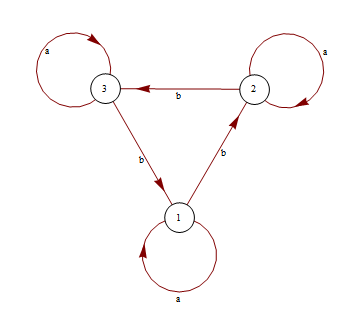
\includegraphics[width=0.7\textwidth]{rysunek8}
    \caption{Automat niesynchroniczny}
    \label{fig:rysunek8}
\end{figure}

Nasuwa si\k{e} wi\k{e}c pytanie, je\'{s}li mamy dany sko\'{n}czony automat $\mathscr{A}=(Q, \Sigma, \delta)$, jak stwierdzi\'{c} czy jest on synchroniczny czy nie?

%% Twierdzenie 4.1
\begin{twr}
\label{tw:twierdzenie1}
Sko\'{n}czony automat $\mathscr{A}=(Q, \Sigma, \delta)$ jest synchroniczny wtedy i tylko wtedy, gdy dla dowolnych stan\'{o}w $q, q' \in Q$ istnieje s{\l}owo $w \in \Sigma$ takie, \.{z}e $\delta(q,w)=\delta(q',w)$.
\end{twr}

Zredukujmy problem z Twierdzenia \ref{tw:twierdzenie1} dotycz\k{a}cego synchronizowalno\'{s}ci automatu do problemu zasi\k{e}gu w automacie par $P^{[2]}(\mathscr{A})$ automatu pot\k{e}gowego $P(\mathscr{A})$, kt\'{o}rego zbi\'{o}r stan\'{o}w jest z{\l}o\.{z}ony z jednoelementowych oraz dwuelementowych podzbior\'{o}w zbioru $Q$. Automat par posiada $\frac{|Q|(|Q|+1)}{2}$ stan\'{o}w. Algorytm BFS, czyli przeszukiwanie grafu wszerz, rozwi\k{a}zuje problem znalezienia s{\l}owa synchronizuj\k{a}cego automat w czasie $O(|Q|^2*|\Sigma|)$. To ograniczenie pozwala wnioskowa\'{c}, i\.{z} je\'{s}li s{\l}owo resetuj\k{a}ce nie istnieje dostaniemy o tym stosown\k{a} informacj\k{e} w sko\'{n}czonej jednostce czasu, kt\'{o}rej wielko\'{s}\'{c} zale\.{z}y od rozmiar\'{o}w zar\'{o}wno zbioru stan\'{o}w jak i alfabetu. Je\'{s}li natomiast automat $\mathscr{A}$ jest synchroniczny, jako wynik algorytmu wyprodukowane zostanie s{\l}owo resetuj\k{a}ce ten automat. Najlepszy znany algorytm, kt\'{o}ry jako wynik daje s{\l}owo resetuj\k{a}ce posiada z{\l}o\.{z}ono\'{s}\'{c} czasow\k{a} rz\k{e}du $O(|Q|^3+|Q|^2*|\Sigma|)$ oraz z{\l}o\.{z}ono\'{s}\'{c} pami\k{e}ciow\k{a} rz\k{e}du $O(|Q|^2*|\Sigma|)$, nie licz\k{a}c pami\k{e}ci potrzebnej na zapisanie wyniku, kt\'{o}ra jest rz\k{e}du $O(|Q|^3)$.


%% SEKCJA 5 Problem długości słowa synchronizującego
\section{Z{\l}o\.zono\'s\'c problemu d{\l}ugo\'{s}ci s{\l}owa resetuj\k{a}cego.}

Automat pot\k{e}gowy synchronicznego automatu mo\.ze by\'c u\.zyteczny w konstruowaniu najkr\'otszych s{\l}\'ow resetuj\k{a}cych, co jest zwi\k{a}zane z najkr\'otsz\k{a} \'scie\.zk\k{a} w automacie pot\k{e}gowym od ca{\l}ego zbioru stan\'ow, a\.z do pojedynczego stanu. Oczywi\'scie w najgorszym przypadku wymaga to wyk{\l}adniczego czasu. Niemniej jednak by{\l}y pr\'oby zaimplemetowania tego podej\'scia. Mo\.zna mie\'c nadziej\k{e}, \.ze odpowiednie obliczenia dla "wielomianowego" subautomatu $P^{[2]}(\mathscr{A})$ pozwol\k{a} uzyska\'c algorytm wielomianowy. Jednak, ma{\l}o prawdopodobne jest to, \.ze istnieje jakikolwiek rozs\k{a}dny algorytm znajdowania najkr\'otszego s{\l}owa resetuj\k{a}cego w przypadku og\'olnym.\\ 
\\
Rozwa\.zmy teraz dwa nast\k{e}puj\k{a}ce problemy:

%% Problem 4.1
\begin{pro}
(Kr\'otkie s{\l}owo resetuj\k{a}ce.) Maj\k{a}c automat synchroniczny  $\mathscr{A}=(Q, \Sigma, \delta)$ i liczb\k{e} naturaln\k{a} $l$, czy prawd\k{a} jest to, \.ze $\mathscr{A}$ posiada s{\l}owo resetuj\k{a}ce o d{\l}ugo\'sci $l$?
\end{pro}

%% Problem 4.2
\begin{pro} (Najkr\'otsze s{\l}owo resetuj\k{a}ce.) Maj\k{a}c automat synchroniczny  $\mathscr{A}=(Q, \Sigma, \delta)$ i liczb\k{e} naturaln\k{a} $l$, czy prawd\k{a} jest to, \.ze minimalna  d{\l}ugo\'s\'c s{\l}owa resetuj\k{a}cego automat $\mathscr{A}$ jesr r\'owna $l$?
\end{pro}

Oczywi\'scie problem 5.1 nale\.zy do klasy z{\l}o\.zono\'sci NP; mo\.zna nie -deterministycznie odgadn\k{a}\'c s{\l}owo $w\in\Sigma^{*}$ o d{\l}ugo\'sci $l$, a nast\k{e}pnie sprawdzi\'c czy $w$ jest s{\l}owem resetuj\k{a}cym automat $\mathscr{A}$ w czasie wielomianowym. David Eppstein udowodni{\l}, w 1990 roku \.ze problem 5.1 jest NP-trudny przez wielomianow\k{a} redukcj\k{e} z problemu NP-zupe{\l}nego. Dlatego problem 5.1 jest NP-zupe{\l}ny. Z dowodu tego {\l}atwo wynika, \.ze problem 5.2 jest NP-trudny. Wojciech Samotij \cite{1} pokaza{\l}, \.ze negacja NP-zupe{\l}no\'sci mo\.ze by\'c wielomianowo zredukowana do problemu 5.2, sk\k{a}d ostatni problem r\'ownie\.z jest coNP-trudny. Jako konsekwencja problem 5.2 nie mo\.ze nale\.ze\'c do klasy NP je\.zeli nieprawd\k{a} jest, \.ze NP=coNP, co jest powszechnie uwa\.zane za ma{\l}o prawdopodobne. Innymi s{\l}owy, nawet nie-deterministyczny algorytm nie mo\.ze znale\'z\'c minimalnej d{\l}ugo\'sci s{\l}owa resetuj\k{a}cego dla danego automatu synchronicznego w czasie wielomianowym.

Z drugiej strony wyczerpuj\k{a}ce przeszukiwanie wszystkich s{\l}\'ow nad alfabetem $\Sigma$ o d{\l}ugo\'sci $\leq l$ mo\.ze zosta\'c wykonane w pami\k{e}ci wielomianowej, a w rzeczywisto\'sci w liniowej. Dlatego problem 5.2 nale\.zy do klasy z{\l}o\.zono\'sci PSPACE. Pytanie o precyzyjne ulokowanie tego problemu w odniesieniu do hierarchii wielomian\'ow wci\k{a}\.z pozostaje otwarte. 

Trudno\'s\'c problemu decyzyjnego w 5.1 implikuje to, \.ze jego zoptymalizowana wersja, w kt\'orej szuka si\k{e} s{\l}owa resetuj\k{a}cego o minimalnej d{l}ugo\'sci dla danego automatu synchronicznego r\'ownie\.z jest trudna. Jednak\.ze to nie wyklucza tego, \.ze problem optymalizacji mo\.ze dopuszcza\.c wielomianowy algorytm aproksymacji, co wi\k{e}cej wszystkie istniej\k{a}ce dowody tego, \.ze problem 5.1 jest NP-trudny s\k{a} zgodne z  przypuszczeniem \.ze taki algorytm istnieje. Orzeczenie czy to przypuszczenie jest prawdziwe, czy te\.z nie stanowi ciekawy problem badawczy. Carl Pixley \cite{2} w 1992 zasugewowa{\l} heurystyczny algorytm znajdowania kr\'otkiego s{\l}owa resetuj\k{a}cego dla automatu synchronicznego, kt\'ory zosta{\l} wykorzystany do wykonywania zadowalaj\k{a}cych ilo\'sci test\'ow. P\'o\'zniej algorytmy szukaj\k{a}ce kr\'otkich s{\l}\'ow resetuj\k{a}cych zosta{\l}y zaimplementowane przez Avrahama Trahtmana \cite{3}.


%% SEKCJA 6 Hipoteza Cernego
\section{Hipoteza \v Cernego.}

W tym rozdziale om\'{o}wimy otwarty do tej pory problem i wyniki, zwi\k{a}zane z nast\k{e}puj\k{a}cym pytaniem: posiadaj\k{a}c zadane $n \in N$ jak d{\l}ugie mo\.ze by\'c s{\l}owo resetuj\k{a}ce sko\'nczony automat synchroniczny o $n$ stanach? 

Przywo{\l}ajmy najpierw konstrukcj\k{e} \v Cernego. Dla liczby naturalnej $n>1$ oznaczmy $C_{n}$ jako sko\'nczony automat synchroniczny, kt\'orego stany s\k{a} resztami modulo $n$, a litery wej\'sciowe $a$ i $b$ dzia{\l}aj\k{a} nast\k{e}puj\k{a}co:\\
\\
$\delta(0,a)=1$\\
$\delta(m,a)=m$ for $0<m<n$\\
$\delta(m,b)=m+1(modn)$
%% Rysunek 
\begin{figure}[H]
    \centering
    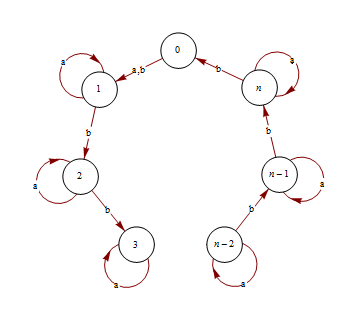
\includegraphics[width=0.8\textwidth]{rysunek7}
    \caption{Automat $C_{n}$}
    \label{fig:rysunek7}
\end{figure}

\v Cerny udowodni{\l}, \.ze $C_{n}$ jest automatem synchronicznym i najkr\'otszym resetuj\k{a}cym go s{\l}owem jest $(ab^{n-1})^{n-2}a$ o d{\l}ugo\'sci $(n-1)^{2}$. Zatem je\'sli zdefiniujemy funkcj\k{e} \v Cernego $C(n)$ jako d{\l}ugo\'s\'c najkr\'otszego s{\l}owa resetuj\k{a}cego automat synchroniczny posiadaj\k{a}cy $n$ stan\'ow powy\.zsza w{\l}asno\'s\'c dla ci\k{a}gu $\{C_{n}\}_{n=2,3,\ldots}$ daje nier\'owno\'s\'c: $C(n)\leq(n-1)^{2}$. Hipoteza \v Cernego m\'owi, \.ze tak naprawd\k{e} zachodzi r\'owno\'s\'c: $C(n)=(n-1)^{2}$. W literaturze mo\.zna spotka\'c nawi\k{a}zania do tego, \.ze praca \v Cernego z 1964 roku jest \'zr\'od{\l}em tej hipotezy, ale tak naprawd\k{e} nie zosta{\l}a ona wtedy sformu{\l}owana. Jednak\.ze \v Cerny zaobserwowa{\l}, \.ze: $(n-1)^{2}\leq C(n)\leq2^{n}-n-1$ i za{\l}\k{a}czy{\l} do tego nast\k{e}puj\k{a}c\k{a} uwag\k{e}: "R\'o\.znica pomi\k{e}dzy granicami wzrasta szybko i nale\.zy je zacie\'sni\'c. Mo\.zna si\k{e} spodziewa\'c polepszenia g{\l}\'ownie dla g\'ornej granicy."

Hipoteza w swej obecnej postaci zosta{\l}a sformu{\l}owana troch\k{e} p\'ozniej, po tym jak oczekiwania zawarte w powy\.zszym cytacie zosta{\l}y potwierdzone przez Peter'a Starke'a \cite{4}, kt\'ory pomniejszy{\l} g\'orn\k{a} granic\k{e} do $1+\frac{n(n-1)(n-2)}{2}$, co by{\l}o pierwsz\k{a} wielomianow\k{a} g\'orn\k{a} granic\k{a} dla $C(n)$. \v Cerny wypowiedzia{\l} hipotez\k{e} $C(n)=(n-1)^{2}$ na Konferencji Cybernetycznej  w Bratys{\l}awie w 1969 roku.


%% SEKCJA 7 Oszacowanie długości słowa synchronizującego z dowodem
\section{Oszacowanie d{\l}ugo\'{s}ci s{\l}owa synchronizuj\k{a}cego.}

W rozdziale sz\'ostym przedstawiona zosta{\l}a tre\'s\'c hipotezy \v Cernego oraz pewne g\'orne oszacowania funkcji $C_{n}$, kt\'ore z  biegiem czasu stawa{\l}y si\k{e} coraz dok{\l}adniejsze. Najdok{\l}adniejsze znane g\'orne ograniczenie funkcji \v Cernego gwarantuje to, \.ze dla ka\.zdego automatu synchronicznego posiadaj\k{a}cego $n$ stan\'ow istnieje s{\l}owo resetuj\k{a}ce o d{\l}ugo\'sci $\frac{n^{3}-n}{6}$. Takie s{\l}owo resetuj\k{a}ce powstaje w wyniku nast\k{e}puj\k{a}cego algorytmu.\\


\textbf{Algorytm 7.1}\\ 
\textbf{wej\'scie}: $\mathscr{A}=(Q, \Sigma, \delta)$\\
\textbf{inicjalizacja}: \\
$w\leftarrow 1$\\ 
$P\leftarrow Q$\\
\textbf{je\'sli} $|P|>1$ to znajd\'z s{\l}owo $v\in\Sigma^{*}$ o minimalnej d{\l}ugo\'sci takie, \.ze $|\delta(P,v)|<|P|$;\\
je\'sli takie s{\l}owo nie istnieje \textbf{zwr\'o\'c}: brak;\\
$w\leftarrow wv$\\ 
$P\leftarrow \delta(P,v)$\\
\textbf{zwr\'o\'c}: w;\\

 
Je\'sli $|Q|=n$ to p\k{e}tla g{\l}\'owna algorytmu 7.1 jest wykonywana co najwy\.zej $n-1$ razy. Dzieje si\k{e} tak w  przypadku gdy w każdej iteracji $|P|-|\delta(P,v)|=1$. W celu oszacowania d{\l}ugo\'sci s{\l}owa wyj\'sciowego $w$ musimy estymowa\'c d{\l}ugo\'s\'c ka\.zdego s{\l}owa $v$ uzyskanego w  p\k{e}tli g{\l}\'ownej. 
Rozwa\.zmy og\'olny krok, w kt\'orym $|P|=k>1$ i za{\l}\'o\.zmy \.ze $v=a_{1}\ldots a_{l}$, gdzie $a_{i}\in \Sigma, i=1,\ldots, l$. {\L}atwo zauwa\.zy\'c, \.ze zbiory $P_{1}=P, P_{2}=\delta(P_{1},a_{1}),\ldots, P_{l}=\delta(P_{l-1},a_{l-1})$ s\k{a} $k$-elementowymi podzbiorami $Q$. Ponadto je\'sli $|\delta(P_{l},a_{l})|<|P_{l}|$, to istniej\k{a} dwa stany $q_{l},q'_{l}\in P_{l}$ takie, \.ze $\delta(q_{l},a_{l})=\delta(q'_{l},a_{l})$. Teraz zdefiniujmy  $2$-elementowe podzbiory $R_{i}=\{q_{i},q'_{i}\}\subseteq P_{i}, i=1,\ldots,l$ takie, \.ze $\delta(q_{i},a_{i})=q_{i+1}, \delta(q'_{i},a_{i})=q'_{i+1}, i=1,\ldots,l-1$. Dla $1\leq i<j\leq l$ $R_{j}\not\subseteq P_{i}$, poniewa\.z wprzeciwnym przypadku istnia{\l}oby s{\l}owo $v'=a_{1}\cdot\ldots\cdot a_{i-1}a_{j}\cdot\ldots\cdot a_{l}$ takie, \.ze $|\delta(P_{k},v')|<|P_{k}|$, co jest sprzeczne z  minimaln\k{a} d{\l}ugo\'sci\k{a} s{\l}owa $v$. Dochodzimy do poni\.zszego, kombinatorycznego problemu.

\begin{pro}
Niech $Q$ b\k{e}dzie $n$-elementowym zbiorem, $P_{1},\ldots,P_{l}$ ci\k{a}giem $k$-elementowych podzbior\'ow zbioru $Q$, $(k>1)$, a $R_{1},\ldots,R_{l}$ ci\k{a}giem $2$-elementowych podzbior\'ow zbioru $Q$. Przypu\'s\'cmy $R_{i}\subseteq P_{i}$ dla ka\.zdego $i=1,\ldots,l$, ale $R_{j}\not\subseteq P_{i}$ dla $1\leq i<j\leq l$. Jak du\.za liczba $l$ mo\.ze by\'c?
\end{pro}

Problem 7.1 zosta{\l} rozwi\k{a}zany przez Petera Frankla w 1982 roku, kt\'ory udowodni{\l} nast\k{e}puj\k{a}ce twierdzenie: 

\begin{twr} 
Niech $A_{1},\ldots,A_{m}$ b\k{e}dzie ci\k{a}giem zbior\'ow o mocy $r$, a $B_{1},\ldots,B_{m}$ b\k{e}dzie ci\k{a}giem zbior\'ow o mocy $s$, spe{\l}niaj\k{a}cych: $A_{i}\cap B_{i}=\emptyset$ dla $i=1,\ldots,m$ oraz $A_{i}\cap B_{j}\neq\emptyset$ dla $i<j$. Wtedy zachodzi nie\'owno\'s\'c:
\begin{equation} 
m\leq{{r+s}\choose{s}}
\end{equation}
\end{twr} 

\begin{proof}[Dow\'od]
Oznaczamy $X=\bigcup_{i=1}^{m} (A_i \cup B_{i})$. X jest zbiorem sko\'nczonym. Wybieramy zbi\'or $V\in\mathbb{R}^{r+1}$, spe{\l}niaj\k{a}cy warunki: 
\begin{enumerate}[1)]
\item $|V|=|X|$ 
\item ka\.zde $r+1$ wektor\'ow z $V$ s\k{a} liniowo niezale\.zne
\end{enumerate}
 Nast\k{e}pnie ka\.zdy element zbioru $X$ nale\.zy powi\k{a}za\'c z odpowiednim elementem zbioru $V$, dzi\k{e}ki czemu zbiory $A_{i}$ oraz $B_{i}$ mo\.zna rozwa\.za\'c jako podzbiory V. Teraz dla ka\.zdego $j$ zdefiniujmy wielomian 
\begin{equation}
f_{j}(x)=\prod_{v\in B_{j}}<v,x> 
\end{equation}
 powi\k{a}zany ze zbiorem $B_{j}$, gdzie $x=(x_{1},\ldots,x_{r+1})$. Skoro $A_{i}$ sk{\l}ada si\k{e} z $r$ liniowo niezale\.znych wektor\'ow, to pow{\l}oka liniowa $A_{i}$ ma wymiar $r$. Pow{\l}oka liniowa zbioru $A_{i}$ jest oczywi\'scie podprzestrzeni\k{a} wektorow\k{a} przestrzeni $\mathbb{R}^{r+1}$, a wi\k{e}c jest te\.z przestrzeni\k{a} wektorow\k{a} nad cia{\l}em $\mathbb{R}$.  Dla ka\.zdego $i$ wybieramy wektor normalny przestrzeni $spanA_{i}$. Oznaczmy go $y_{i}$. Wektor $y_{i}$ jest prostopad{\l}y do przestrzeni $spanA_{i}$, wi\k{e}c $<v,y_{i}>=0$, je\'sli tylko $v\in spanA_{i}$.\\ 
Poka\.zemy \.ze $v\in spanA_{i}$, je\'sli $v\in A_{i}$. Przypu\'s\'cmy, \.ze $v\in spanA_{i}$, ale $v\notin A_{i}$. Zauwa\.zmy \.ze $span(A_{i}\cup\{v\})=spanA_{i}$, gdzie $spanA_{i}$ ma wymiar $r$. Zatem $span(A_{i}\cup\{v\})$ r\'ownie\.z ma wymiar $r$, co jest sprzeczne z za{\l}o\.zeniem, \.ze dowolne $r+1$ wektor\'ow z $V$ s\k{a} liniowo niezale\.zne. \\
Mamy zatem \.ze $<v,y_{i}>=0$, je\'sli $v\in A_{i}$. Wiemy zatem, \.ze $f_j(y_{i})=0$ je\'sli $<v,y_{i}>=0$ dla pewnego $v\in B_{j}$. Ponadto $<v,y_{i}>=0$ dla pewnego $v\in B_{j}$, je\'sli $v\in B_{j}$ i $v\in A_{i}$, co zachodzi w przypadku, gdy $A_{i}\cap B_{j}\neq\emptyset$. Z za{\l}o\.ze\'n wiemy, \.ze $A_{i}\cap B_{j}\neq\emptyset$ dla $i<j$ oraz $A_{i}\cap B_{j}=\emptyset$ dla $i=j$. Zatem $f_{j}(y_{i})=0$ dla $i<j$ oraz $f_{j}(y_{i})\neq0$ dla $i=j$. \\
Teraz poka\.zemy, \.ze $\{f_{j}\}_{j=1}^{m}$ tworz\k{a} uk{\l}ad liniowo niezale\.zny. Przypu\'s\'cmy, \.ze tak nie jest. Istnieje zatem $k$, takie \.ze: $c_{k}\neq0$ oraz zachodzi r\'owno\'s\'c: 
\begin{equation}
 c_{1}f_{1}+\ldots+c_{k}f_{k}+\ldots+c_{m}f_{m}=0
\end{equation} 
Rozwa\.zmy warto\'s\'c powy\.zszej kombinacji liniowej na wektorze $y_{k}$: 
\begin{equation}
c_{1}f_{1}(y_{k})+\ldots+c_{k}f_{k}(y_{k})+\ldots+c_{m}f_{m}(y_{k})=0 
\end{equation}
$\forall i$ $i<k$: $f_{i}(y_{k})=0$. Poza tym, na podstawie powy\.zszych rozwa\.za\'n mamy: $\forall_{i}$ $i>k$: $f_{i}(y_{k})=0$. Tym samym z r\'ownania znikaj\k{a} wszystkie sk{\l}adniki, poza jednym. Otrzymujemy $c_{k}f_{k}(y_{k})=0$. Ale wiemy \.ze $f_{k}(y_{k})\neq0$. Zatem $c_{k}=0$, co jest sprzeczne  z za{\l}o\.zeniem $c_{k}\neq0$.\\
Udowodnili\'smy, \.ze $\{f_{j}\}_{j=1}^{m}$ tworz\k{a} uk{\l}ad liniowo niezale\.zny. Teraz musimy ograniczy\'c wymiar podprzestrzeni zawieraj\k{a}cej $\{f_{j}\}_{j=1}^{m}$. Dla ka\.zdego $j$ wszystkie jednomiany wielomianu $f_{j}$ maj\k{a} stopie\'n $s$ i tworz\k{a} baz\k{e} tej podprzestrzeni. Ka\.dy jednomian stopnia $s$ ma posta\'c $x_{1}^{l_{1}}\cdot\ldots\cdot x_{r+1}^{l_{r+1}}$, gdzie $l_{1}+\ldots+l_{r+1}=s$. Musimy teraz odpowiedzie\'c na nast\k{e}puj\k{a}ce pytanie: jak du\.zo r\'o\.znych jednomian\'ow tej postaci istnieje? Rozwi\k{a}zaniem tego problemu dla nieujemnych $l_{1},\ldots,l_{r+1}$ jest liczba ${r+s}\choose{s}$. Zatem $\{f_{j}\}_{j=1}^{m}$ jest uk{\l}adem $m$-liniowo niezale\.znych element\'ow, zawartym w przestrzeni o wymiarze mniejszym b\k{a}d\'z r\'ownym ${r+s}\choose{s}$. Otrzymujemy tez\k{e} twierdzenia: $m\leq{{r+s}\choose{s}}$.
\end{proof}

Teraz tez\k{e} twierdzenia 7.1, wykorzystujemy do rozwi\k{a}zania problemu 7.1. Skoro dla ka\.zdego $i$ $R_{i}\subseteq P_{i}$ to $\forall_{i}$ $(Q-P_{i})\cap R_{i}=\emptyset$ oraz $|Q-P_{i}|=n-k$. Ponadto je\.zeli $R_{j}\not\subseteq P_{i}$ dla $1\leq i<j\leq l$, to dla $1\leq i<j\leq l$ zachodzi $(Q-P_{i})\cap R_{j}\neq\emptyset$. Przyjmujemy: $A_{i}=Q-P_{i}$, $r=n-k$, $B_{i}=R_{i}$, $s=2$, $m=l$ i podstawiaj\k{a}c do wzoru otrzymanego w twierdzeniu otrzymujemy: $l\leq$ ${n-k+2}\choose{2}$. Wiemy, \.ze p\k{e}tla algorytmu wykona si\k{e} maksymalnie $n-1$ razy w wyniku czego otrzymamy s{\l}owo resetuj\k{a}ce postaci: $w=w_{1}\ldots w_{n-1}$. Zatem, aby dosta\'c g\'orne ograniczenie d{\l}ugo\'sci s{\l}owa resetuj\k{a}cego nale\.zy posumowa\'c $l\leq{{n-k+2}\choose{2}}$ po $k=2,..,n$. Ostatecznie mamy: 
\begin{equation}
\sum_{k=2}^{n}{{n-k+2}\choose{2}}=\frac{n^{3}-n}{6}
\end{equation}



\begin{thebibliography}{99}
\bibitem{1} W. Samotij: A note on the complexity of the problem of finding shortest synchronizing words.
\bibitem{2} C. Pixley: Exact calculation of synchronization sequences based on decision diagrams.
\bibitem{3} A. Trahtman: An efficient algorithm finds noticeable trends concerning the \v Cern\'y conjecture.
\bibitem{4} P. H. Starke: Eine Bemerkung \H uber homogene Experimente, Elektronische Informationverarbeitung und Keybernetic.
\end{thebibliography}

\end{document}
